 \chapter{Simulation sous Orcad Spice}
  \section{Circuit}
    Vu les performances de l’algorithme, on partira de celui-ci pour les valeurs, et 
    on affinera directement grâce à SPice.

   \subsection{Page principale}
    Puisque notre amplificateur est composé de quatre étages indépendants, nous avons décidé d'utiliser quatre "pages"
    différentes, ainsi qu'une "page"  principale, regroupant les différents circuits précédents, afin d'y voir plus clairement.

    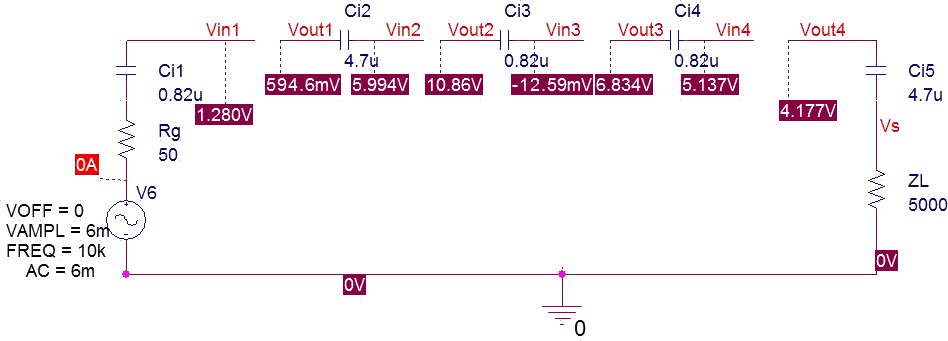
\includegraphics[width=17cm]{images/g}

    On choisit les autres condensateurs de manière à nous assurer une fréquence de coupure voisine de 100 \hertz.

   \subsection{Premier étage : Collecteur Commun}
    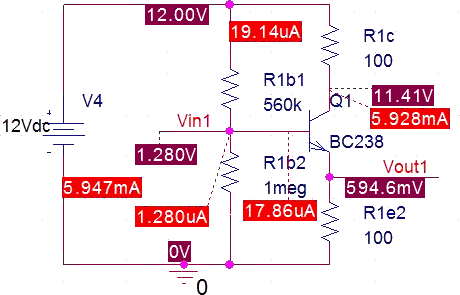
\includegraphics[width=17cm]{images/1}

   \subsection{Deuxième étage : Émetteur Commun}
    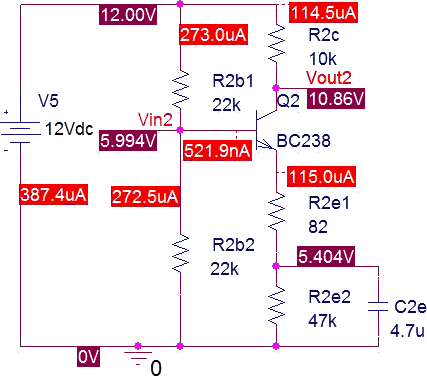
\includegraphics[width=17cm]{images/2}

   \subsection{Troisième étage : Amplificateur Différentiel}
    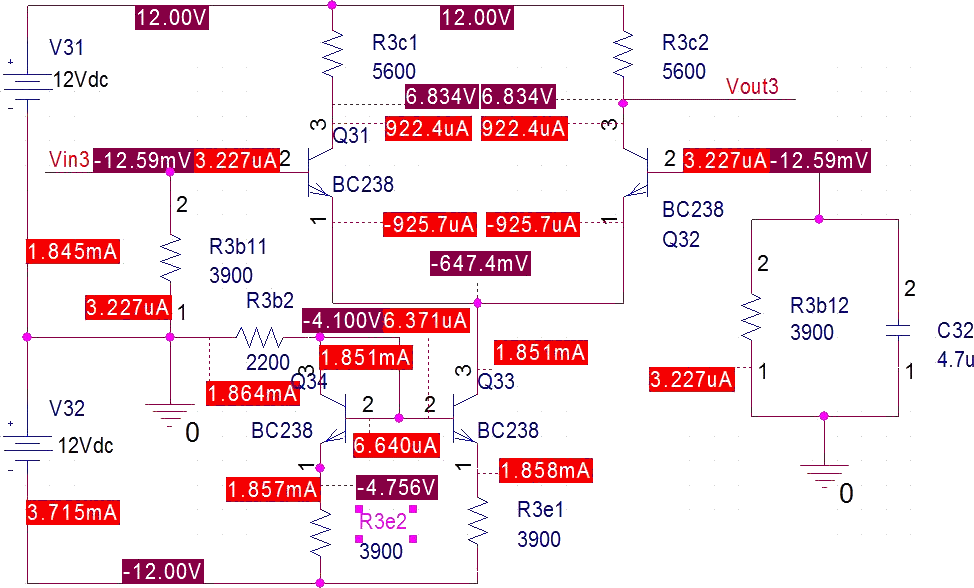
\includegraphics[width=17cm]{images/3}

   \subsection{Quatrième étage : Collecteur Commun}
    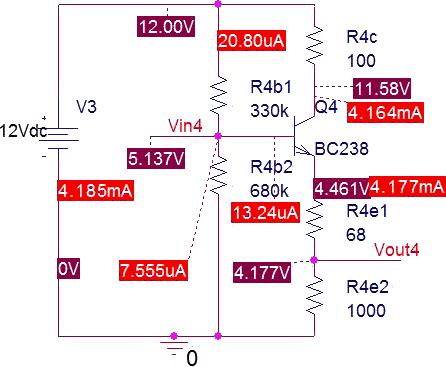
\includegraphics[width=17cm]{images/4}

  \section{Simulation}
   \subsection{Diagramme de Bode}
    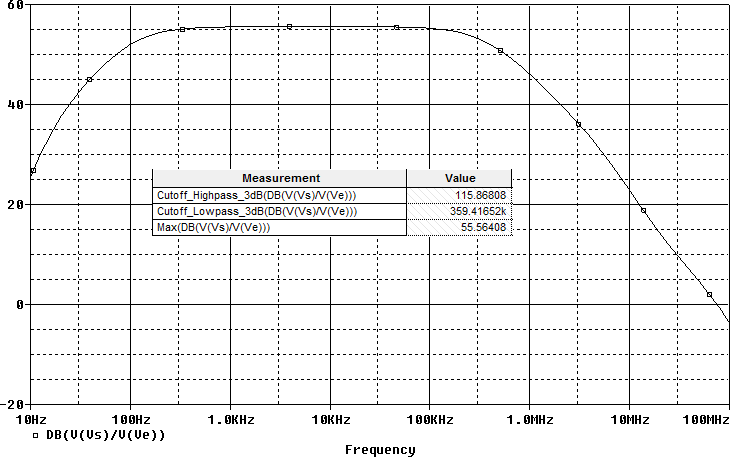
\includegraphics[width=17cm]{images/bode}

  \section{Respect du cahier des charges}
   Voici les caractéristiques principales de notre amplificateur, telles que données par
   Spice, qui complètent les données de polarisation présentes sur les schémas:

   \subsection{Fréquences de coupure}
    Ces fréquences sont données par Spice avec les fonctions \verb|Cutoff_Lowpass_3dB()| et \verb|Cutoff_Highpass_3dB()| :

    $F_{CBF} = 115$ \hertz

    $F_{CHF} = 359$ \kilo\hertz

   \subsection{Impédances d'entrée et de sortie}
    En traçant un "diagramme de Bode" sous Spice avec, pour chaque étage, $\cfrac{V_E}{I_E}$, on obtient (à 30 \kilo\hertz):
    \begin{itemize}
     \item $Z_{E_1} = \verb|32030|\ohm = Z_E$ : On respecte bien le cahier des charges.
     \item $Z_{E_2} = \verb|9644|\ohm$
     \item $Z_{E_3} = \verb|3294|\ohm$
     \item $Z_{E_4} = \verb|124060|\ohm$
    \end{itemize}

    Pour l'impédance de sortie, il faut modifier un peu le circuit sous spice : court-circuiter l'entrée et déplacer le générateur à la place de la charge. On obtient alors :
    \begin{itemize}
     \item $Z_{S_3} = \verb|5435|\ohm$
     \item $Z_{S_4} = \verb|85|\ohm = Z_S \Rightarrow$ Contrairement à ce que nous avions prévu, nous n'ajouterons pas de résistance série.
    \end{itemize}

   \subsection{Gain et dynamique de sortie}
    On obtient un gain de \verb|55,56| dB, soit une amplification de 600.
    Notre dynamique de sortie est de \verb|6,09012|\volt.
   \subsection{Distorsion harmonique}
    Toujours d'après Spice : \verb|TOTAL HARMONIC DISTORTION =   4,509345E+00 PERCENT|

   \subsection{Courants de collecteur}
    \begin{itemize}
     \item $I_{C_1} = 5,928 \milli\ampere$
     \item $I_{C_2} = 0,114 \milli\ampere$
     \item $I_{C_3} = 0,926 \milli\ampere$
     \item $I_{C_4} = 4,164 \milli\ampere$
    \end{itemize}

   \subsection{Amplitudes crête à crête}
    \begin{itemize}
     \item $A_1 =$ \verb|11,34| \milli\volt
     \item $A_2 =$ \verb|90,94| \milli\volt
     \item $A_3 =$ \verb|6,67| \volt
     \item $A_4 =$ \verb|6,09| \volt
    \end{itemize}
